%====================================================================================
\section[Intercambio]{Intercambio puro}
%====================================================================================

\begin{frame}{Ejemplo}
	Jaime y Karen tienen un total de 10 unidades de alimentos y 6 unidades de ropa.
	\begin{table}
		\begin{tabular}{|c|c|c|c|}
			\hline
			Agentes & Asignación inicial & Intercambio & Asignación final \\
			\hline
			Jaime & 7A, 1R & -1A, +1R & 6A, 2R\\
			\hline
			Karen & 3A, 5R & +1A, -1R & 4A, 4R\\
			\hline
		\end{tabular}
	\end{table}
	Para saber si estan mejor es necesario conocer sus preferencias por alimentos y comida.
\end{frame}
%------------------------------------------------
\begin{frame}{Ejemplo}
	\begin{itemize}
		\item Karen tiene mucha ropa y poco alimento
		\begin{itemize}
			\item Supongamos que la RMS de alimento por ropa es 3.
			\item Para conseguir 1 unidad adicional de alimento tiene que renunciar a 3 unidades de ropa.
		\end{itemize}
		\item Supongamos que la RMS de Jaime de comida por ropa es solo de $\frac{1}{2}$.
		\begin{itemize}
			\item Estará dispuesto a renunciar a $\frac{1}{2}$ unidad de alimento por 1 unidad adicional de ropa.
		\end{itemize}
	\end{itemize}
\end{frame}
%------------------------------------------------
\begin{frame}{Ejemplo}
	\begin{itemize}
		\item Existen condiciones para el intercambio
		\begin{itemize}
			\item Jaime valora la ropa más que Karen
			\item Karen valora el alimento más que Jaime.
			\item Karen estará dispuesta a renunciar hasta 3 unidades de ropa para conseguir 1 unidad adicional de alimento, pero Jaime solo renunciará a $\frac{1}{2}$	 unidad de ropa por una unidad adicional de alimento
		\end{itemize}
		\item Los términos del intercambio se determinan a través de la negociación.
		\begin{itemize}
			\item El intercambio de 1 unidad de alimento se realizará a cambio de entre $\frac{1}{2}$ y 3 unidades de ropa.
		\end{itemize}
	\end{itemize}
\end{frame}
%------------------------------------------------
\begin{frame}{Ejemplo}
	\begin{itemize}
		\item Supongamos que Karen ofrece a Jaime 1 unidad de ropa por 1 unidad de alimento.
		\begin{itemize}
			\item Jaime tendrá más ropa, que él valora más que el
			alimento.
			\item Karen tendrá más alimento, que ella valora más que 	la ropa.
		\end{itemize}
		\item Siempre que las RMS de dos consumidores sean diferentes hay oportunidad para el intercambio mutuamente beneficioso.
		\begin{itemize}
			\item La asignación de los recursos es ineficiente.
		\end{itemize}
	\end{itemize}
\end{frame}
%------------------------------------------------
\begin{frame}{Introducción}
	Clasificación de los Modelos de equilibrio general
		\begin{itemize}
			\item Según el poder de mercado de los agentes:
				\begin{itemize}
					\item Equilibrio general competitivo
					\item Equilibrio general con oligopolios
				\end{itemize}
			\item Según cómo se considere a los bienes:
				\begin{itemize}
					\item Equilibrio general de intercambio puro
					\item Equilibrio general con producción
				\end{itemize}
		\end{itemize}
\end{frame}
%------------------------------------------------
\begin{frame}{Descripción de la economía}
	\begin{itemize}
		\item Mercancías
		\item Un conjunto de consumidores
			\begin{itemize}
				\item Preferencias
				\item Dotación inicial de recursos ($w$)
				\item Conjunto de consumo ($X$)
			\end{itemize}
		\item Un conjunto de empresas
			\begin{itemize}
				\item Tecnología
			\end{itemize}
	\end{itemize}
\end{frame}
%------------------------------------------------
\begin{frame}{Definiciones previas}
	\begin{itemize}
		\item Economía de intercambio
			\begin{itemize}
				\item Es una proyección del conjunto de consumidores sobre el espacio de características de los agentes.
				\item Problema de los agentes: cómo redistribuir los recursos iniciales de la mejor forma posible.
				\item Posibles decisiones:
					\begin{itemize}
						\item Consumir sus dotaciones iniciales
						\item Involucrarse en un proceso de intercambio de sus recursos iniciales para diseñar una canasta de consumo mejor.
						$$\begin{array}{lcl}
							\hspace{-1cm} \text{Economía de trueque} & \longrightarrow & \text{Núcleo de una economía} \\
							\hspace{-1cm} \text{Subastador de precios} & \longrightarrow & \text{Equilibrio walrasiano}
						\end{array}$$
					\end{itemize}
			\end{itemize}
		\item Asignación
			\begin{itemize}
				\item Es una función que a cada consumidor $i$ asocia una canasta de consumo $x_i$
			\end{itemize}
		\item Asignación factible
			\begin{itemize}
				\item Es una asignación tal que la cantidad agregada de bienes se iguala a la cantidad agregada de dotaciones iniciales
					$$\sum x_i = \sum w_i$$
			\end{itemize}
	\end{itemize}
\end{frame}
%------------------------------------------------
\begin{frame}{Definiciones previas}
	\begin{itemize}
		\item Asignación eficiente
			\begin{itemize}
				\item Una asignación factible para una economía es eficiente (Pareto-óptima) si no hay una asignación factible alternativa que permite mejorar a un agente sin que otro agente empeore
					\begin{gather*}
						\widehat{x} \text{ es eficiente si} \\
						\sum \widehat{x}_i = \sum w_i \\
						\nexists x_{i}^{\prime} : \sum x_{i}^{\prime} = \sum w_i \text{ y } x_{i}^{\prime} \succ^{i} \widehat{x}_i,\enskip \forall i
					\end{gather*}
			\end{itemize}
		\item Racionalidad individual
			\begin{itemize}
				\item Una asignación $x_i$ satisface la propiedad de racionalidad individual si el consumidor $i$ está dispuesto a intercambiar su dotación inicial $w_i$ por una asignación $x_i$ que le proporciona mayor satisfacción.
			\end{itemize}
		\item Coalición
			\begin{itemize}
				\item Una coalición $S$ es un subconjunto del conjunto de consumidores
			\end{itemize}
	\end{itemize}
\end{frame}
%------------------------------------------------
\begin{frame}{Definiciones previas}
	\begin{itemize}
		\item Mejor asignación para una coalición
			\begin{itemize}
				\item Una coalición $S$ puede mejorar sobre una asignación (bloquear) $x$ , si existe una asignación alternativa y para $S$ tal que, sea factible para la coalición y también sea preferida para todos los miembros de la coalición.
					\begin{gather*}
						y_i \succ^{i} x_i \enskip , \enskip \forall i\\
						\sum y_i = \sum w_{y}
					\end{gather*}
			\end{itemize}
		\item Núcleo de la economía
			\begin{itemize}
				\item El núcleo es el conjunto de las asignaciones factibles sobre las que ninguna coalición $S$ puede mejorar.
			\end{itemize}
	\end{itemize}
\end{frame}
%------------------------------------------------
\begin{frame}{El modelo de intercambio puro}
	\begin{itemize}
		\item 	Modelo de intercambio puro: el caso especial de los modelos de EG en el que todos los agentes económicos son consumidores e intercambian sus dotaciones iniciales de los bienes.
		\item Demandante neto de un bien (oferente): el consumidor quiere consumir más (menos) que su dotación inicial de ese bien.
	\end{itemize}
\end{frame}
%------------------------------------------------
\begin{frame}{intercambio puro: 2 agentes y 2 bienes}
	\begin{itemize}
		\item \textbf{Ventaja}
		\begin{itemize}
			\item No hay producción: los bienes existentes en la economía porque sí. Son variables exógenas.
			\item Dos bienes, $1$ y $2$.
			\item Dos consumidores o economías domésticas.
		\end{itemize}
	\end{itemize}
\end{frame}
%------------------------------------------------
\begin{frame}{2 agentes y 2 bienes: Dotaciones y Cestas}
	\begin{itemize}
		\item \textbf{Novedad}: Los consumidores no tienen rentas sino bienes
			\begin{itemize}
				\item Dos consumidores: $A$ y $B$
				\item Dos bienes: $x_1$ y $x_2$
				\item Las dotaciones iniciales:
					\begin{itemize}
						\item $w^{A}=(w_{1}^{A},w_{2}^{A})$
						\item $w^{B}=(w_{1}^{B},w_{2}^{A})$
					\end{itemize}
				\item Sus consumos:
					\begin{itemize}
						\item $x^{A}=(x_{1}^{A},x_{2}^{A})$
						\item $x^{B}=(x_{1}^{B},x_{2}^{B})$
					\end{itemize}
				\item Sin intercambio:
					\begin{itemize}
						\item $x^{A}=w^{A}$
						\item $x^{B}=w^{B}$
					\end{itemize}
				\item Con intercambio, muchas situaciones pueden ocurrir, pero lo siguiente es una asignación factible o viable si
					\begin{itemize}
						\item $x_{1}^{A}+x_{1}^{A}=w_{1}^{A}+w_{1}^{B}$
						\item $x_{2}^{B}+x_{2}^{B}=w_{2}^{B}+w_{2}^{B}$
					\end{itemize}				
			\end{itemize}
	\end{itemize}
\end{frame}
%------------------------------------------------
\begin{frame}{2 agentes y 2 bienes: Funciones de utilidad}
Cada agente posee unas preferencias bien definidas sobre las cestas de bienes y puede consumir su dotación inicial o intercambiarla con otros agentes (trueque)\\
	\bigskip
\textbf{Preferencias de las economías domésticas:}
	\begin{itemize}
		\item Función de utilidad consumidor A:\quad $u^{A}(x_{1}^{A},x_{2}^{A})$
		\item Función de utilidad consumidor B:\quad $u^{B}(x_{1}^{B},x_{2}^{B})$
	\end{itemize}
\end{frame}
%------------------------------------------------
\begin{frame}{2 agentes y 2 bienes: Funciones de utilidad}
		Función de utilidad del agente A\\
			\vspace{0.5cm}
		\centering
			\begin{tikzpicture}[transform canvas={scale=0.6}]
	% Formato de CAJA
		\draw[->] (0.5,0.5) node[align=center, below left] {\footnotesize $O_A$} -- (0.5,4.5) node[align=center, above] {\footnotesize $K^{A}$};
		\draw[->] (0.5,0.5) -- (8.5,0.5) node[align=center, right] {\footnotesize $L^{A}$};
	
		% Curvas de indiferencia1
			% Agente B
				\draw  [blue] (0.6,4) ..controls (1.4,1.4) and (1.74,1) .. (6,0.6);
				\draw  [blue] (1,4.3) ..controls (1.7,2.1) and (2,1.6) .. (6.3,1);
				\draw  [blue] (1.6,4.6) ..controls (2.1,3.2) and (1.74,2.2) .. (6.7,1.4);
			
			% Flechas
				\node[draw, single arrow,
						minimum height=30mm, minimum width=1mm,
						single arrow head extend=1.5mm,
						anchor=west, blue, fill=blue, scale=0.5, rotate=50] at (2.7,2.7) {};
	
	% Formato de CAJA rotado
		\draw[->] (18,4) node[align=center, above right] {\footnotesize $O_B$} -- (10,4) node[align=center, left] {\footnotesize $L^{B}$};
		\draw[->] (18,4) -- (18,0) node[align=center, below] {\footnotesize $K^{B}$};
	
		% Curvas de indiferencia1
			% Agente B
				\draw [red] (12,3.9) .. controls (16.76,3.5) and (17.1,3.1) .. (17.9,0.5);
				\draw [red] (11.7,3.5) .. controls (16.5,2.9) and (16.8,2.4) .. (17.3,0.2);
				\draw [red] (11.3,3.1) .. controls (16.76,2.3) and (16.4,1.3) .. (16.6,-0.1);
			
			% Flechas
				\node[draw, single arrow,
						minimum height=30mm, minimum width=1mm,
						single arrow head extend=1.5mm,
						anchor=west, red, fill=red, scale=0.5, rotate=-130] at (15.7,1.8) {};
\end{tikzpicture}
\end{frame}
%------------------------------------------------
\begin{frame}{2 agentes y 2 bienes: Funciones de utilidad}
	Función de utilidad del agente B\\
		\vspace{3.5cm}
	\hspace{-0.5cm} \vspace{-0.5cm}
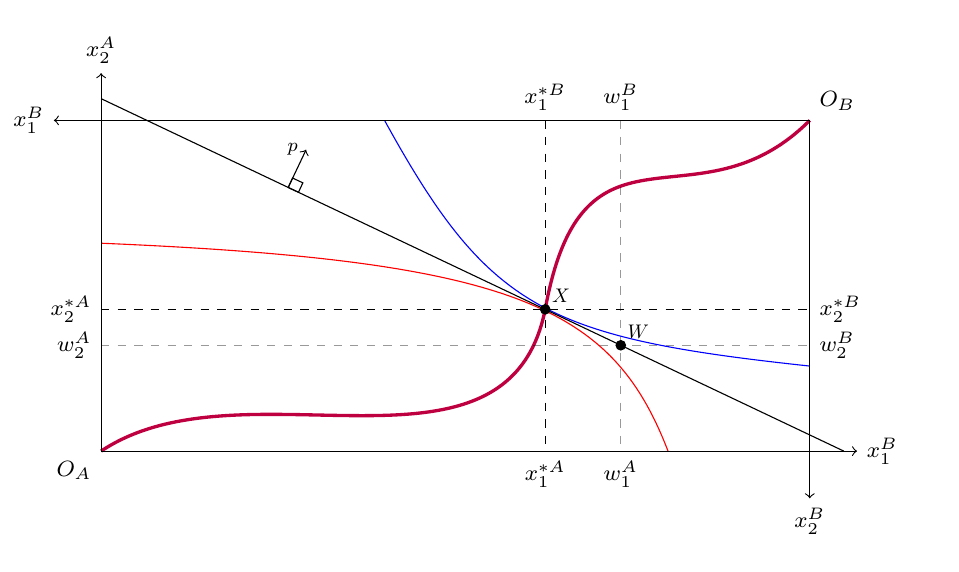
\begin{tikzpicture}[scale=1.2]
	\hspace{-0.3cm}
	% Curva de contrato 5.2,2
		\draw  [purple, very thick] (0.5,0.5) ..controls (2,1.5) and (4.8,0) .. (5.2,2) ..controls (5.6,4.2) and (6.8,2.8) .. (8,4);
	% Intersección de una dotación
		% Demanda: x
			\draw[dashed] (5.2,4) node[above] {\footnotesize $x_{1}^{*B}$} -- (5.2,0.5) node[below]{\footnotesize $x_{1}^{*A}$};
			\draw[dashed] (0.5,2) node[left] {\footnotesize $x_{2}^{*A}$} -- (8,2)node[right]{\footnotesize $x_{2}^{*B}$};
		
		% Oferta: w
			\draw[dashed, opacity=0.4] (6,4) -- (6,0.5);
			\draw[dashed, opacity=0.4] (0.5,1.62)  -- (8,1.62);
			
			\draw (8,1.62)  node [right] {\footnotesize $w_{2}^{B}$};
			\draw (6,4)  node [above] {\footnotesize $w_{1}^{B}$};
			
			\draw (0.5,1.62)  node [left] {\footnotesize $w_{2}^{A}$};
			\draw (6,0.5)  node [below] {\footnotesize $w_{1}^{A}$};
	
	% Curvas de indiferencia
		\draw [blue] (3.5,4) .. controls (4.6,2) and (5.2,1.7) .. (8,1.4);
		\draw [red] (0.5,2.7) .. controls (4.915,2.515) and (5.915,2.015) .. (6.5,0.5);
	
	% Recta presupuestaria
		\draw (0.5,4.23) -- (8.36,0.5);
	
	% Puntos
		\draw[black, fill=black] (5.2,2) circle[radius=0.05] node [above right, scale=0.25mm] {$X$};
		\draw[black, fill=black] (6,1.62) circle[radius=0.05] node [above right, scale=0.25mm] {$W$};
	
	% Flecha y rectángulo
		\draw [->] (2.48,3.29) -- (2.67,3.69) node [left, scale = 0.3mm] {\footnotesize $p$};
		\draw [rotate around={-25:(2.48,3.29)}] (2.48,3.29) rectangle (2.6, 3.4);
		
	% Formación de la caja
		% Consumidor A
			\draw[->] (0.5,0.5) node[align=center, below left] {\footnotesize $O_A$} -- (0.5,4.5) node[align=center, above] {\footnotesize $x_{2}^{A}$};
			\draw[->] (0.5,0.5) -- (8.5,0.5) node[align=center, right] {\footnotesize $x_{1}^{B}$};
		
		%Consumidor B
			\draw[->] (8,4) node[align=center, above right] {\footnotesize $O_B$} -- (0,4) node[align=center, left] {\footnotesize $x_{1}^{B}$};
			\draw[->] (8,4) -- (8,0) node[align=center, below] {\footnotesize $x_{2}^{B}$};
\end{tikzpicture}
\end{frame}